%<dscrpt>Introduction à la dynamique de la fonction logistique</dscrpt>
L'objet de ce problème est l'étude des suites définies par une valeur initiale $x_0$ et
\[
\forall n \in \N, \; x_{n+1}=f_{\mu}(x_n)
\]
où $f_\mu$ (appelée fonction \emph{logistique}) est définie par:
\[
\forall x \in \R, \; f_\mu (x)=\mu x(1-x).
\]
Le paramètre $\mu$ est strictement positif, on pose aussi $c_\mu = \frac{\mu -1}{\mu}$. \newline
On dira qu'un intervalle $I$ de $\R$ est stable lorsque :
\[ 
x\in I \Rightarrow f_\mu (x)\in I.
\] 
On demande plusieurs fois d'étudier $(x_n)_{n\in\N}$ en discutant suivant $x_0$.  Il s'agit de former une liste d'intervalles et de décrire le comportement de la suite lorsque $x_0$ est dans chacun des intervalles listés. On devra justifier ces descriptions.

\subsection*{Partie I}
\begin{enumerate}
\item Quels sont les points fixes de $f_\mu$ ?
\item Former le tableau de variation de $f_\mu$, préciser le maximum absolu et la valeur de la fonction en ce point.
\item Calculer $f_\mu ^\prime (0)$ et $f_\mu ^\prime (c_\mu)$. Comparer suivant la valeur de $\mu$ ces valeurs avec $-1$ et $+1$.  Que peut-on en déduire ?
\item Pour quelles valeurs de $\mu$ l'intervalle $[0,1]$ est-il stable ?
\item Les quatre figures \ref{fig:Elogistic_1}, \ref{fig:Elogistic_2}, \ref{fig:Elogistic_3}, \ref{fig:Elogistic_4} présentent les graphes de $f_\mu$ pour quatre valeurs de $\mu$ parmi $0.7$, $1.7$, $2.7$, $4.7$. Indiquer sur la feuille au dessous de chaque dessin le $\mu$ correspondant et placer le $c_\mu$ sur l'axe des abscisses. 
\end{enumerate}

\subsection*{Partie II}
Dans cette partie, lorsque $\mu>2$, on notera $S_\mu = [\frac{1}{2},\frac{\mu}{4}]$ et $K_\mu =\max _{S_\mu}|f_\mu ^\prime|$.
\begin{enumerate}
\item\begin{enumerate}
 \item En calculant d'abors la valeur pour $\mu=2$, factoriser $f_\mu(\frac{\mu}{4})-\frac{1}{2}$. 
\item Factoriser $f'_\mu(\frac{\mu}{4})+1$.
\end{enumerate}

\item Cas $\mu \in \left]0,1\right[$. \'Etudier $(x_n)_{n\in\N}$ en discutant suivant $x_0$.
\item Cas $\mu \in \left]1,2 \right[$. \'Etudier $(x_n)_{n\in\N}$ en discutant suivant $x_0$.
\item Montrer que $\mu \in \left]2,1+\sqrt{5} \right[$ entraîne $S_\mu$ stable.
\item On suppose ici que $\mu \in \left]2,1+\sqrt{3}\right[$.
\begin{enumerate}
 \item Montrer que $S_\mu$ est stable et que $K_\mu < 1$.
\item Montrer que $x_0\in S_\mu$ entraîne
\[
\forall n\in \N, \; |x_n - c_\mu|\leq K_\mu ^n |x_0 - c_\mu|.
\]
 \item Montrer que si $x_0\in \left]0,\frac{1}{2} \right]$, il existe $k\in \N$ tel que $x_k\in S_\mu$. Que peut-on en déduire ?
\end{enumerate}

\end{enumerate}

\subsection*{Partie III. Vers un ensemble de Cantor}
\begin{figure}[ht]
\begin{center}
	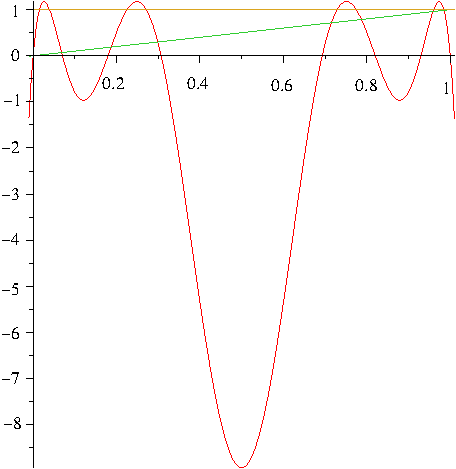
\includegraphics{Elogistic_5.pdf}
\end{center}
\caption{$\mu=4.73 \: :\; f_\mu \circ f_\mu \circ f_\mu$}
\label{fig:Elogistic_5}
\end{figure}
On se place cette fois dans le cas $\mu>2+\sqrt{5}$. Pour tout entier $n$, $f_\mu ^n$ désigne la composée de $f_\mu $ par elle même $n$ fois. Voir figure \ref{fig:Elogistic_5} par exemple. On note aussi :
\begin{displaymath}
\Lambda_n = \{x\in\R , f_\mu ^n(x)\in [0,1]\} \hspace{1cm}
\Lambda = \bigcap_{n\in \N} \Lambda _n .
\end{displaymath}

($f_\mu ^0$ désigne l'identité de $\R$.)
\begin{enumerate}
\item Préciser les $u\in[0,1]$ tel que $f_\mu (u)=1$. En déduire $\Lambda_1$.
\item L'intervalle $[0,1]$ est-il stable ? Pour quels $x_0$ la suite $(x_n)_{n\in\N}$ prend-elle toutes ses valeurs dans $[0,1]$.
\item Montrer que si $f_\mu (u)=1$ alors $|f_\mu ^\prime(u)|>1$ .
\item Soit $\lambda=\inf_{\Lambda_1}|f_\mu ^\prime|$. Montrer que $\lambda >1$ .
\item Montrer que $\Lambda_{n+1}\subset\Lambda_n$. Montrer que $\Lambda_n$ est formé par $2^n$ intervalles disjoints.
\item \begin{enumerate}
\item Montrer que pour tout $x\in \Lambda_n$ :
\[
|(f_\mu ^n)^\prime(x)|\geq \lambda ^n .
\] 
\item Montrer que la longueur de chaque intervalle formant $\Lambda_n$ est inférieure à $\dfrac{1}{\lambda^{n+1}}$.
\end{enumerate}
\end{enumerate}
\clearpage
\begin{figure}[p]
 \centering
 \input{Elogistic_1.pdf_t}
 \caption{Partie I. 5}
 \label{fig:Elogistic_1}
\end{figure}
\begin{figure}[p]
 \centering
 \input{Elogistic_2.pdf_t}
 \caption{Partie I. 5}
 \label{fig:Elogistic_2}
\end{figure}
\begin{figure}[p]
 \centering
 \input{Elogistic_3.pdf_t}
 \caption{Partie I. 5}
 \label{fig:Elogistic_3}
\end{figure}
\begin{figure}[p]
 \centering
 \input{Elogistic_4.pdf_t}
 \caption{Partie I. 5}
 \label{fig:Elogistic_4}
\end{figure}
\clearpage


